\documentclass[11pt,psfig]{article}
\usepackage{epsfig}
\usepackage{times}
\usepackage{amssymb}
\usepackage{float}

\newcount\refno\refno=1
\def\ref{\the\refno \global\advance\refno by 1}
\def\ux{\underline{x}}
\def\uw{\underline{w}}
\def\bw{\underline{w}}
\def\ut{\underline{\theta}}
\def\umu{\underline{\mu}} 
\def\bmu{\underline{\mu}} 
\def\be{p_e^*}
\newcount\eqnumber\eqnumber=1
\def\eq{\the \eqnumber \global\advance\eqnumber by 1}
\def\eqs{\eq}
\def\eqn{\eqno(\eq)}

 \pagestyle{empty}
\def\baselinestretch{1.1}
\topmargin1in \headsep0.3in
\topmargin0in \oddsidemargin0in \textwidth6.5in \textheight8.5in
\begin{document}
\setlength{\parskip}{1.2ex plus0.3ex minus 0.3ex}


\thispagestyle{empty} \pagestyle{myheadings} \markright{G}



\title{CS 266 Homework 7}
\author{Zachary DeStefano, PhD Student, 15247592}
\date{Due Date: May 29, 2014}

\maketitle

\vfill\eject

\section*{Problem 7.7}
Do the breakpoints of the beach line always move downwards when the
sweep line moves downwards? Prove this or give a counterexample.\\
\\
This is true. If we look at the existing breakpoints that are above the sweep line, they are the intersections of parabolas that represent the region where it's closer to the points than to the sweep line. If you move the sweep line down, then no points will get deleted from this region, but points will be added to the bottom of it, thus the parabolas move downward and their intersections would thus have to move down since the parabolas move uniformly. 

\section*{Problem 7.11}

Let P be a set of n points in the plane. Give an O(nlogn) time algorithm
to find for each point p in P another point in P that is closest to it.\\
\\
Here is the algorithm:\\
1. Compute the Voronoi Diagram\\
2. For the cell of p:\\
Find perpendicular distance to each edge of p\\
Figure out which is closer and the corresponding point is the closest one to p\\
\\
Running time:\\
There are n cells\\
There are $O(n)$ edges total since the storage required is $O(n)$ thus the checking step takes a total of $O(n)$ time. \\
Computing the Voronoi Diagram will take $O(n \cdot log(n))$ time. \\
Total running time is thus $O(n \cdot log(n))$

\section*{Problem 9.11}

A Euclidean minimum spanning tree (EMST) of a set P of points in the
plane is a tree of minimum total edge length connecting all the points.
EMST’s are interesting in applications where we want to connect sites
in a planar environment by communication lines (local area networks),
roads, railroads, or the like.\\

\subsection*{Part a}
Prove that the set of edges of a Delaunay triangulation of P contains
an EMST for P.\\
\\
Make the Euclidean tree. \\
Apply Kruskal's to get an MST. \\
Because the Delaunay Triangulation gets all the sets of points which are closest together, all the edges for them will be included. 

\subsection*{Part b}
Use this result to give an O(nlogn) algorithm to compute an EMST
for P.\\
Compute the Delaunay Triangulation. \\
Apply Kruskal's algorithm to the graph derived from the triangulation to get the EMST\\

\section*{Problem 9.17}

The weight of a triangulation is the sum of the lengths of all edges of
the triangulation. A minimum weight triangulation is a triangulation
whose weight is minimal. Disprove the conjecture that the Delaunay
triangulation is a minimum weight triangulation.\\
\\
If we take a quadrilateril that points inward, then we can construct a case where the Delaunay triangulation will have greater weight than the minimum weight triangulation.

\begin{figure}[H]
\centering
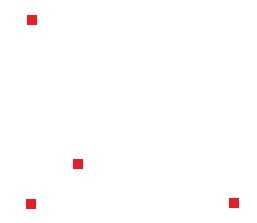
\includegraphics[height=2.5in]{hw7prob3diagram1.jpg}
\caption{The Four Points to Triangulate}
\end{figure}

\begin{figure}[H]
\centering
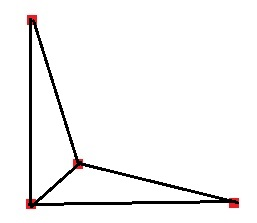
\includegraphics[height=2.5in]{hw7prob3diagram2.jpg}
\caption{The Minimum Weight Triangulation}
\end{figure}

\begin{figure}[H]
\centering
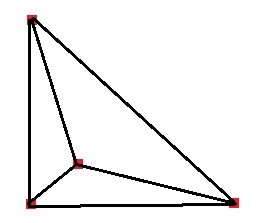
\includegraphics[height=2.5in]{hw7prob3diagram3.jpg}
\caption{The Delaunay Triangulation}
\end{figure}

\end{document}








